

\documentclass{article}
\usepackage{graphicx}
\usepackage{color}

\sloppy
\definecolor{lightgray}{gray}{0.5}
\setlength{\parindent}{0pt}

\begin{document}

    
    \begin{verbatim}
function [ ] = Sinus()

x=(-pi:0.001:4*pi);

f=figure(1);

title('Sinus and squarewave')
axis('auto')
q=plot(x,sin(x)), xlabel('time (x values)'), ylabel('y'), grid on

set(q,'Color','green','LineWidth',2)

legend('sin(x)', 'square(x)')

hold on

for i=1:length(x)

if sin(x(i))<0

wave(i)=-1;

else

wave(i)=1;

end

end

p=plot(x,wave)

set(p,'Color','red','LineWidth',2)

end
\end{verbatim}

        \color{lightgray} \begin{verbatim}
q =

  416.0011


p =

  417.0011

\end{verbatim} \color{black}
    
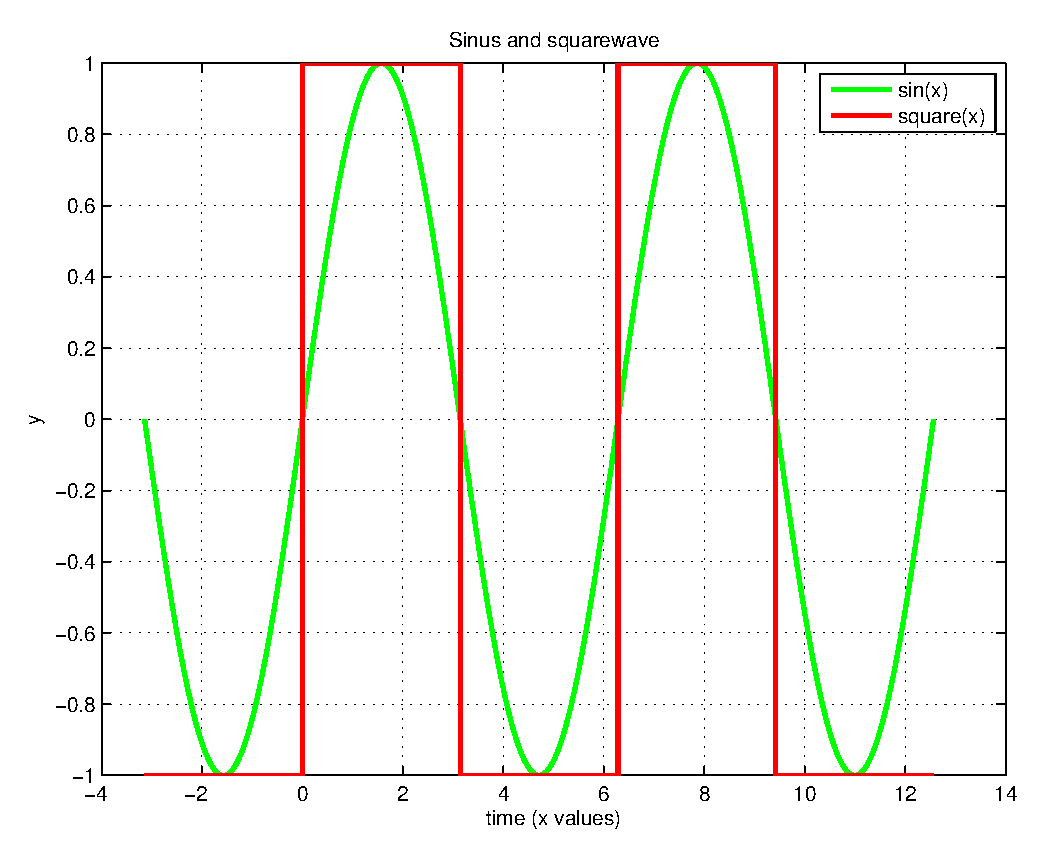
\includegraphics [width=4in]{Sinus_01.eps}



\end{document}
    
